\documentclass{aifyp}

\usepackage{multicol}
\usepackage{cite}
\usepackage{graphicx} \usepackage[bottom]{footmisc}
\usepackage[section]{placeins} \raggedbottom{}
\usepackage{amsmath}
\usepackage{graphicx}
\usepackage{listings}
\usepackage[hidelinks]{hyperref}
\usepackage{float}
\usepackage{qtree}
\usepackage{array,hhline}
\usepackage[ruled,vlined]{algorithm2e}

\usepackage{pdflscape}
\usepackage{afterpage}


\title{Automatic User Profiling for Intelligent
Tourist Trip Personalisation} 
\author{Liam Attard}

\graphicspath{ {./assets/} }

\supervisor{Dr Josef Bajada}
\date{June 2021} 

\longabstract{

     The objective of holiday activity planning is to maximise the
    traveller's enjoyment during such trips by selecting the right places to
    visit and things to do according to the person's preferences. This process
    involves preparing information from various data sources, which is often
    very time-consuming. This project presents a tourist itinerary
    recommendation algorithm that assists users by autonomously generating a
    personalised holiday plan according to the user's travel dates and
    constraints.  Furthermore, the system automatically builds a travel
    interest profile from the user's social media presence, which is then used
    to recommend itineraries tailored to the user's interests. The system uses
    social media APIs from popular platforms such as Facebook and Instagram.
    With the user's permission, the system gathers information such as pages
    the user likes and pictures posted by the user. 

    A Convolution Neural Network  is used to classify the user's pictures into their respective
    travel category, such as Beach, Clubbing, Nature, Museums or Shopping,
    which is then used to determine the user's predominant travel interest
    topics. A Resnet-18, Resnet-50 and Keras Sequential model are validated 
    separately on a testing dataset to see which one works best.  This computed
    travel profile of a user takes the form of a weight vector, which is then
    used to generate an automated itinerary that fits the user's preferences
    and travel constraints. 

    This weight vector is used to formulate a
    personalised objective function used by various meta-heuristic and
    evolutionary algorithms to optimise the plan. The algorithms consider hard
    constraints such as holiday dates, distances between places, and soft
    constraints (preferences), such as the interests and the user's preferred
    pace. This dissertation compares Particle Swarm Optimisation and Genetic
    Algorithms, and they are evaluated for both their plan quality and
    performance.

Since the results are highly personalised, the system was packaged into an
application that allows users to connect with their social media accounts,
build a personalised travel plan for a holiday in Malta, and ask the user to
assess the plan's quality with respect to personal preferences and activity pace. The
user is also asked to assess a more generic holiday itinerary without
specification of the generated plan, in order to assess the
effectiveness of the personalised holiday planning algorithm. }

\acknowledgement{I want to thank the following people for helping with this research project:

First, I would like to thank Dr Josef Bajada for guiding me positively
throughout this dissertation and always making me feel confident in my
abilities. Second, I would also like to thank Kelcy De Marco for all her patience, love
and support. Finally, I would like to thank my parents, siblings and friends
who have supported and motivated me consistently throughout this project.}

\begin{document} 


\pagenumbering{roman}
\tableofcontents 
\clearpage{\pagestyle{empty}}

\listoffigures 
\clearpage{\pagestyle{empty}}

\listoftables 
\clearpage{\pagestyle{empty}}

\pagenumbering{arabic} 
\setcounter{page}{1}


\section{Introduction}
\label{Introduction}

\subsection{Problem Definition}
Leisure travelling is an impactful industry
whose economic importance significantly improves each
year, contributing to 10.4\% of the global GDP in 2019
~\cite{wttc2018travel}. Despite this, planning for a trip to a
foreign city requires a substantial amount of
time-consuming research. As a result, people often
rely on multiple data sources such as travel
brochures, blogs and vlogs to form a holiday plan and
retrieve the top-rated points of interests (POI) of a site. 
However, a tourist has to compile a timetable
independently even though mediums do not hold the
resources to provide POIs tailored according to the
traveller's preferences and constraints
~\cite{DeChoudhury2010}. 

In literature, offering tourists a personalised route
composed of POIs has been defined as the tourist trip
design problem (TTDP). The TTDP comprises ranking
and selecting POIs that might interest the user and
create a feasible plan. Figure~\ref{TTDP} shows an example
of the TTDP,  where a tourist has to form a timetable
that balances between the POI's rating and location
while satisfying the various trip constraints. 
The TTDP is an NP-hard problem where rigorous
%TODO: ask about rigorous
algorithms only manage to optimise with a small number
of POIs. Therefore, many approximate algorithms,
namely heuristics and meta-heuristic approaches, work
%TODO: ask about this
to converge solutions with complex alternatives to
this problem.Section
~\ref{Literature} provides a detailed review of this problem and its
variants.  


Nevertheless, the few existing systems that provide
users with an itinerary or route require a lengthy
process of manually gathering the users' likes and
constraints or information from past trips. Therefore, we ask the following question: 


\begin{center}

    \textit{Can a system automatically get to know
    what a tourist likes to visit and use this
information to generate a personalised itinerary for a
holiday?}

\end{center}


\begin{figure}[h]
\centering
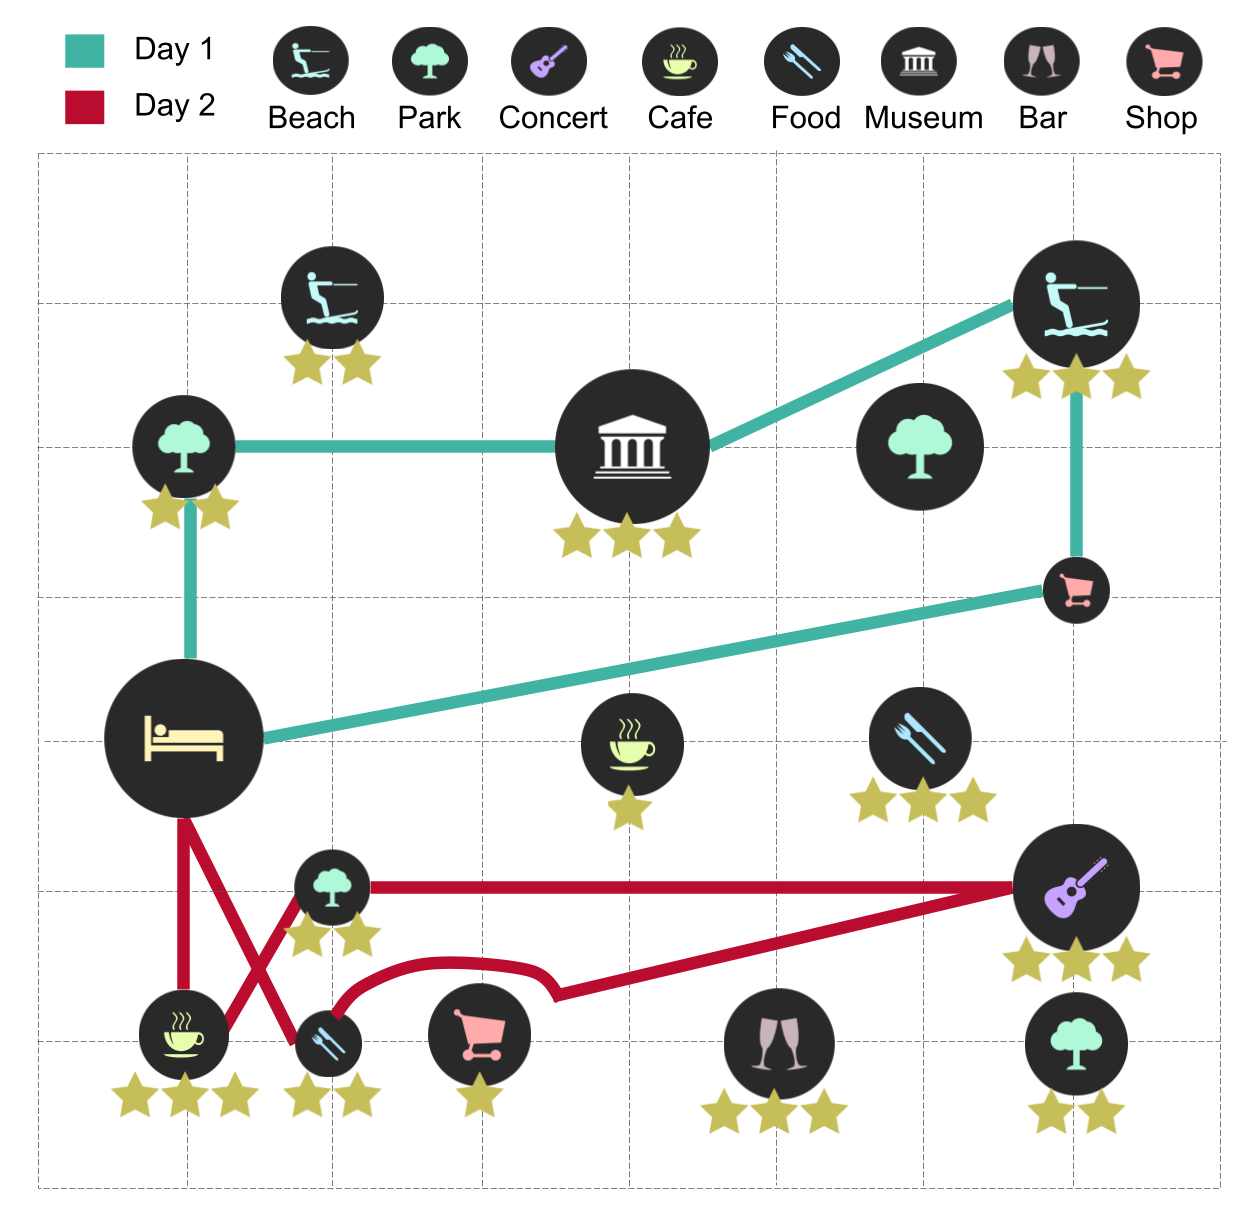
\includegraphics[width=0.65\textwidth]{TTDP.png}
\caption{Example of a tourist planning problem}
\label{TTDP}
\end{figure}

\subsection{Proposed Solution}

To address this problem, we present an application
that helps tourists travel by providing them with a
complete itinerary for their upcoming holiday using
several optimisation algorithms, namely, Genetic
Algorithms (GA) and Particle Swarm Optimisation (PSO).

With the prevalence of social media and data-driven
approaches, we also automate gathering users' POI
desires by scanning their social media profile using
machine learning classification approaches through
Convolutional Neural Networks (CNN).

The results from the evaluation section~\ref{evaluation}
show that we were able to classify the user's photos
and liked pages into a travel interest vector that automatically
describes the user's characteristics. We were also able to provide optimisation
techniques that converge to the timetables with the
best scores given a set of tourist constraints.
In-depth semi-structured interviews with several
participants continued to provide us with further
detail on the accuracy of the user profiling algorithm
and the resulting timetables. 

\subsection{Motivation}

Our primary motivation behind this work is to
introduce the automatic retrieval of user preferences
for other travel planning applications. Currently,
there is no mainstream application that provides
tourists with a fully personalised plan with a quick
and easy to use application.  We were also motivated
by the idea of delivering one centralised system which
organises the whole holiday rather than having to
spend time searching through the excessive amount of
data online. This approach is better than bombarding
potential tourists with many questions to understand
the users' personalities.

\subsection{Why the problem is non-trivial}

Existing algorithms and tourist planners use
heuristics to optimise solutions for the timetable
problem and achievable results in polynomial time
\cite{Vansteenwegen2011}.

Collecting the users' preferences is a
beneficial technique used by businesses to advertise
their products by targeting only a specific audience
\cite{article}.

The problem is non-trivial since we combine both
technologies to provide one system.

\subsection{Aims and Objectives}

This dissertation aims to build an application that
generates a personalised holiday plan according to the
user's travel dates and constraints.


\begin{itemize}
    \item \textbf{Objective 1 (O1)}: Investigate techniques to build travel interest
    profiles automatically from social media interactions.  
    \item \textbf{Objective 2 (O2)}: Explore different optimisation algorithms for
    building personalised travel itineraries using the
    generated travel interest profiles. 
    \item \textbf{Objective 3 (O3)}: Evaluate the
    performance of the personalised travel itinerary
    generator with real users through in-depth
    semi-structured interviews. 

\end{itemize}

We will conduct the interviews by generating a
personalised and non-personalised timetable for a
holiday in Malta to have prior knowledge of the POIs
and compare the effects of both itineraries.

\subsection{Document Structure}

This dissertation is structured as follows; Section~\ref{Literature}
discusses related work relating to existing TTDP
solutions and automatic user preference gathering.
Section~\ref{MethodologyPage} demonstrates the steps taken to create the
whole application along with its underlying mechanism.
Section~\ref{evaluation} will evaluate the performance of the
convolutional neural networks, the optimisation
algorithms and discuss the interview's outcomes.
Finally, section 5 will address the findings obtained
from this research concerning the objectives and some
future improvements.



\pagebreak

\section{Background Research and Literature Review}

This section aims to position our study and ease the understanding of its
conclusions and implications.  Therefore, the upcoming sections describe work
related to the technologies that we will use in this dissertation. In the first
part, we provide an overview of the TTDP research area. We then describe
methods of retrieving POIs from a location, existing user-profiling techniques
and existing research regarding itinerary generation.

\subsection{Recommender Systems} 

We introduce the term Recommender Systems (RS) as a solution for the TTDP and
present background knowledge and relevant work that forms this thesis's basis.
RSs hold use cases in diverse fields, such as e-commerce, media, and
tourism~\cite{Herzog2020}. However, in tourism, RSs offer tourists information
in a unified and centralised manner, providing them with a plan for their trip
~\cite{Santamaria-Granados2020, DiBitonto2010a, Lim2018}.  Two domains develop
current RSs for the TTDP solutions, which are; methods for obtaining tourist
products (such as events and Point of Interests (POI)) and tour recommendation
algorithms that create tourist trips~\cite{Lim2018} as shown in Figure \ref{RS}.  The following sections
discuss related work in each field and discuss adding personalisation to RSs.

\begin{figure}[h]
\centering
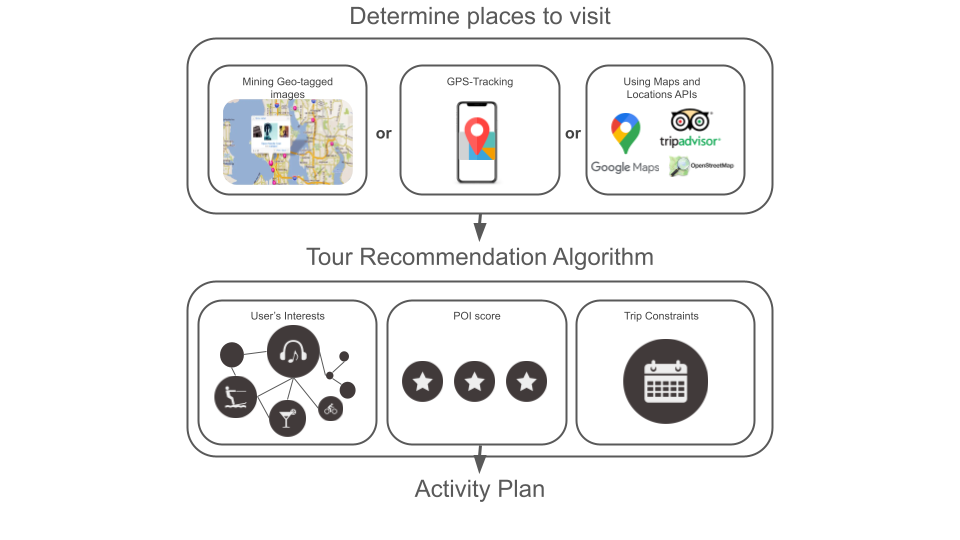
\includegraphics[width=0.8\textwidth]{RSProcess.png}
\caption{Recommender System Process in Tourism}
\label{RS}
\end{figure}

\subsection{Methods of retrieving travel products}

Before producing an itinerary, RSs have to formulate a dataset of POIs from
some data source. The proposed tour recommendation algorithm will then evaluate
a guided path, route or itinerary from this dataset after understanding the
users' implicit preferences such as the travel date and activity moderation. There are several ways to identify an appropriate
data source representing real-life tourist trajectories.  


\paragraph{Geotag mining:} One approach is made by gathering tourist products by mining them from
geotagged images of Location-Based Social Networks (LSBN) such as Flickr,
Facebook or Twitter~\cite{DeChoudhury2010, Memon2015, Lucchese2012, Lim2018a,
HuiLim, HuiLima, Kurashima2013, Kurashima2010, Brilhante2013, Brilhante2015 }.
Lim et al.~\cite{Lim2018} denote this process into three steps; 


\begin{enumerate}

\item First, the application assembles an organised series of relevant
    photographs of the user's destination from the LSBN.\@

\item The application then maps these pictures with a list of popular places
    extracted from sites like Wikipedia.

\item Since the photos contain metadata, like the location and the timestamps;
    the application can calculate an approximate visit duration for each
    specific POI.\

\end{enumerate}

\paragraph{GPS-based data sources:}
The ubiquitous presence of smartphones and
GPS-enabled devices has facilitated
another approach to collecting trajectories~\cite{10.1145/1889681.1889683,
10.1145/1526709.1526816, Chen2011a}. A system
can automatically gather the best POIs to visit based on other users'
historical paths providing additional information such as the average time
people spend at a specific POI and how many people go there. However, privacy
issues are the main caveat towards this approach since it requires people to
share their location constantly and publically\cite{Lim2018}.

\paragraph{Prebuilt dataset:} The most straightforward method is done by self-defining the POIs or gathering
them from a dataset such as the TSPLIB95~\footnote{Sample instances for
travelling salesman Problem:
http://comopt.ifi.uni-heidelberg.de/software/TSPLIB95/}. Manually collecting
travel products provides precision and a better understanding of the itinerary
that the algorithm will generate. However, the algorithm would be
dataset-specific testified and personalised towards what the authors of the
dataset think are the best POIs to visit in a location~\cite{Chou2021a,
Wisittipanich2020, Erbil}.

\paragraph{Maps APIs:} A prompt and accurate strategy towards gathering essential places in the
vicinity is using Mapping \& Location APIs such as Foursquare, Google or
TripAdvisor. Wörndl et al.\cite{Worndl2017} use this approach and build a
dataset of prominent POIs by querying their API with the user's desired location.
In return, they receive a sequence of places and information about each site,
including its category, other user's ratings, opening hours, coordinates and
helpful additional information to use as criteria for the itineraries. However,
the API does not return the average amount of time people spend at a specific
POI.Wörndl et al.\cite{Worndl2017} solve this issue by adding a fixed time
constant for each category with a variable dependant on the POI's score. For
example, suppose a restaurant's time constant is 45 minutes, and the chosen
restaurant has a high score (based on its rating and user's characteristics).
In that case, the time spent at the restaurant will increase by an additional
15 minutes. A significant advantage of using this approach is that the vast
number of POIs that these endpoints return. According to Google's website, the
API contains up to 200 million places with 25 million updates daily which an
application can achieve with a few REST requests\cite{iltifat2014generation, googleSite}.




\subsection{Automatic User Preference Gathering}

User profiles are a virtual representation of a user
containing their characteristics~\cite{Cufoglu}. In
addition, some tourist planners make use of a
technique to personalise the results of their
system~\cite{Worndl2017, Lim2018a, Tumas2009,
Gavalas2015}. For example, Wörndl et al.
\cite{Worndl2017} required the upcoming tourists to
their preferences manually by rating one of six
categories on a scale of 0 to 5: \textit{Sights and Museums,
Night Life, Food, Outdoors and Recreation, Music and
Events and Shopping}. Including a manual input of user
preferences resulted in high user satisfaction since
their timetable was very customised.

\subsubsection{Automatic preference gathering in Travel Planning Applications}

In 2018, Lim et al.\cite{Lim2018a} demonstrated how
implementing personalisation in their algorithm,
PersTours, helped portray real-life scenarios more
accurately. The authors built a system where the
tourist’s level of interest in a specific category is
dependant on their time spent at such POIs, relative
to the average user. First, they gathered information
from the user’s past trips from the social media
platform Flickr. Then, they evaluated their algorithm
using the Root-Mean-Square Error (RMSE), representing
the time deviation of past trips and PersTours results
from Flickr. Although their results show the PersTours
outperforms other applications that use
frequency-based user interest, this approach requires
users to use Flickr and post information about their
past trips on the platform.
 
Nguyen et al.\cite{Nguyen2018} developed an Android
chat application called STSGroup that gathers user’s
preferences and resolves conflicts between tourists by
understanding the messages sent in a group chat. They
provided an example of students travelling to South
Tyrol (Italy), which gathered information such as the
users’ mood and recommended POIs from their
conversations. Other users in the group chat rate
their suggestions through a voting system as the
system uses raking and logistics to calculate
the ideal group preferences in the background. As a
result, 86.7\% of the test users showed satisfaction
with the suggestions.  

\subsubsection{Automatic preference gathering through social media}

The average internet user has gone from being a
passive content absorber to a content producer through
social media. TTDP solutions can use this advantage
and provide a fully automated activity plan based on
the user's characteristics. The following are some
methods for user profiling and information gathering
from the user's social media. 


Instagram has a significant effect on the tourism
industry. Sharing photos of amazing sights and
landscapes influence the way people choose their
POIs\cite{Terttunen2017}. Therefore, a system that
uses tourist's social media photos could infer the
user's preference.

Guntuku et al.~\cite{Guntuku2017} performed an
analysis on the relationship between a user's
characteristics and online images. They found that the
media on the social media profile can predict the big
five personality traits; conscientiousness,
extraversion, neuroticism, agreeableness and openness.
The performance graded by the Pearson correlations
tests were 0.530 and 0.566 for prognosticating
neuroticism and conscientiousness, respectively.

Chen et al.\cite{Chen2013} produced a system for
automatically retrieving tags from images and
incomplete tags called \emph{FastTag}. The algorithm
uses two simple linear mappings. Figure ~\ref{fasttag}
shows an example of an input image used alongside the
\emph{snow, lake, and feet} alongside the incomplete
input tags. In addition, the algorithm produced the
additional tags; \emph{mountain, water, legs, boat,
trees}. 


\begin{figure}[h]
\centering
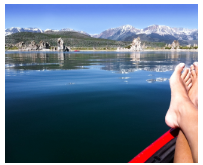
\includegraphics[width=0.4\textwidth]{Fastag}
\caption{Example of an image input for the FastTag algorithm}
\label{fasttag}
\end{figure}

These approaches show how image classification
techniques could provide an automatic preference
gathering system.

\subsection{Travel Planners for both individual and grouped travellers}

This section will focus on breaking down existing meta-heuristic approaches,
notably swarm-based, trajectory-based and evolutionary algorithms, towards the
vast number of variants of the TTDP.\@ Gavalas et al. (Gavalas 2014) classify
these variants into two; Systems that produce a single route and systems that
can handle multiple days. 


\subsubsection{Single Route Problems}

The Orienteering Problem (OP), introduced by Tsiligirdes~\cite{Tsiligirides1984},
in observance of the sport, orienteering, is the foundation of single route planners. 
Figure~\ref{variants} shows the variants of the OP that will be discussed in
this section and how they relate with the original problem.
TTDPs~\cite{Herzog2020}. Vansteenwegen et al.~\cite{Vansteenwegen2011b} describe
OP as a travelling salesman problem with profits. In OP, several nodes $V$
representing POIs where \{$V= {v_1,\ldots,v_n}$\}, are designated in a space
$G$ and edge set $E$ with a starting and an ending
point. Each node holds a score $s$ calculated from the tourist's constraints
and the distance from node $v_i$ to $v_j$. The
objective is to visit a subset of these locations, maximising the $s$ by
obeying the tourist's constraints and minimising the travel
time~\cite{Sylejmani2017}. Vansteenwegen et al.~\cite{Vansteenwegen2011}
mathematically formulate the OP and the methodology contains a mathematical formulation
of this instance of the TTDP.\@
% TODO: (Include Short Maths Formula, maybeone done by Kobeaga2018)


\begin{figure}[h]
\Tree [.{Orienteering Problem (Single Route)} {\ldots} .{Op with Time Windows}  {Time-Dependent OP} 
[{\ldots} ].{Team OP (Multi-Route)} !{\qframesubtree} ]
\caption{Graph showing the variants that will be discussed in the section}
\label{variants}
\end{figure}



%\centering
%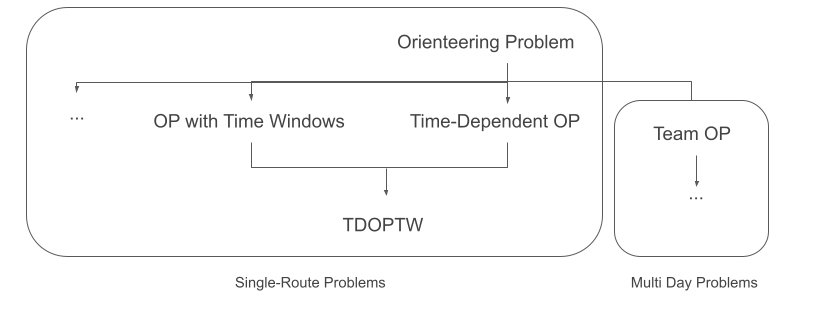
\includegraphics[width=0.5\textwidth]{TOP_graph.png}

Particle Swarm Optimisation-based (PSO) systems provide prevalent OP solutions
with fast computing time. These are bio-inspired meta-heuristic approaches in
which, in the TTDP, a particle represents a travel path. The particles aim to
optimise themselves by communicating with each other and using their velocity
property to move to the most optimal solution~\cite{RezaeeJordehi2013}. In 2010, Sevkli
et al.~\cite{Sevkli2010,Sevkli2010a} tested out two PSO variants:
Strengthened Particle Swarm Optimization (StPSO) and Discrete Strengthened
Particle Swarm Optimization (DStPSO). These two algorithms introduce pioneering
particles, which first perform a local search-based technique called Reduce
Variable Neighborhood Search (RVNS) between all the particles and then assign a
random velocity. These PSO algorithms obtains either the best or competitive
solutions compared with other algorithms such as ant colony and genetic
algorithms when tested on the Tsiligirides~\cite{Tsiligirides1984, Chen2011a} dataset.


There are numerous Evolutionary Algorithms (EA) proposed to solve OP.\@
~\cite{Kobeaga2018,Wang2008}. EAs are algorithms based on natural evolution which
use a fitness score to get to the best solution of a problem, in this case, the
TTDP~\cite{Gunawan2016}. A novel approach in 2018  by Kobeaga et al.~\cite{Kobeaga2018} was able
to find ambitious solutions for over 400 POI nodes using the steady-state
genetic algorithm. The algorithm also implements a local
search, which aims to reduce travel time. 

In 2019, Santini et al.~\cite{Santini2019} introduced a heuristic algorithm based on
adaptive extensive neighbourhood search. They evaluated their system by
comparing it with Kobeage et al.'s EA.\@ The results showed that both algorithms
find suitable solutions in a reasonable amount of time. However, the EA finds
slightly more suitable solutions, while the extensive neighbourhood search has
a lower average gap.

In real-life scenarios, POIs have time constraints that allow them to be
visited only during specific hours, such as opening and closing hours or public
holiday constraints. Traditional OP is not able to cater for such problems. A
single route variant of the OP which solves these issues is the Orienteering
Problem with Time Windows (OPTW)~\cite{Gavalas2014a}. 

Kantor et al.~\cite{Kantor1992} provided the first attempt towards the
OPTW~\cite{Vansteenwegen2011}. They developed two heuristics;
Insertion and depth-first search. The former algorithm solves the path by
selecting a POI with the highest score over-insertion cost incrementally. On
the other hand, the depth-first search algorithm gathers parallel tree-based
solutions simultaneously and iteratively adds new POIs as long as they follow a
set of constraints. Their evaluation showed significant improvements of the
second algorithm over the insertion. Most of the novel solutions of OPTW are
for the multiple route problems discussed in the upcoming sections. 

When travelling between two POIs, the travel time may depend on certain
variable time constraints such as the traffic levels and waiting time~\cite{Herzog2020}.
The Time-Dependent Orienteering Problem (TDOP) introduced by Fomin et al.
~\cite{Fomin2002} is the single route variant of OP, which considers
these scenarios since traditional OP does not~\cite{Gunawan2016}. In 2011, Abbaspour et
al.~\cite{Abbaspour2011}provide a solution for the
Time-Dependent Orienteering Problem with Time Windows, which combines the two
previously mentioned OP variants (TDOPTW).  They propose two adaptive genetic
algorithms and multi-modal shortest pathfinding evaluated in the city of
Tehran.

In 1998, Glover et al.~\cite{Glover1998} introduced a meta-heuristic approach called the
Tabu Search, and several RSs used this algorithm
~\cite{Tang2005,Sylejmani2012,Chou2021}. This optimisation technique is
advantageous when trying to escape
from a local optimum~\cite{Chou2021}. A novel approach by Chou et al.~\cite{Chou2021} aims at
tackling the Probabilistic Orienteering Problem (POP)~\cite{POP}, which
is another variant in which every path contains a cost, and the system can
access every node within a specific probability. Moreover, each node will be
available for a visit only with a certain probability. When evaluated, a simple
tabu search could compete with complex meta-heuristics showing its potential in
this field.



\subsubsection{Multiple Route Problems.}

The RSs available from what we discussed in the previous sections can only
generate a single efficient path for a tourist's holiday. The Team Orienteering
Problem (TOP)~\cite{Chao1996} is a variant of the OP, which allows for
solving the TTDP with multiple days~\cite{Sylejmani2017}. The system generates a full
itinerary for the tourist, with a maximum total score of all routes~\cite{Herzog2020}.

Several Recommender Systems use PSO-based solutions to solve the TOP
~\cite{Muthuswamy2011,Wisittipanich2020,Yu2019}
Muthuswamy et al.~\cite{Muthuswamy2011} developed a discrete version of the PSO (DPSO)
which can generate n routes
where n can be between two to four. The algorithm consists of two procedures;
Random initialisation of n-1 routes with a calculated initialisation of the nth
route based on partial randomness and the current score divided by the current
distance of the particle.  Updating the current velocity of each particle.  The
particles use RVNS and 2-opt techniques to communicate with each other as local
search techniques. The authors evaluated their work by comparing the algorithm
to seven TOP heuristics in which DPSO performed competitively across all
applied benchmark data sets~\cite{Gavalas2014a}.

A few years later, Dang et al.\ wrote another PSO inspired algorithm (PSOiA) for
the TOP.\@ They evaluated their work using an interval graph model, which showed
how to examine a more extensive search space faster~\cite{Gunawan2016}.

Besides swarm-based algorithms, A RS by Sylejmani et al.~\cite{Sylejmani2012}
used the trajectory-based tabu search to solve a Multi Constrained Team OPTW.\
Their system followed three steps in order to generate an activity plan: a new
activity is added as a node to the trip using \emph{Insert}, a node is
exchanged with a new activity using \emph{Replace} and two nodes swap with each
other using \emph{Swap}. 

Several RSs also use PSO-based solutions in novel approaches. For example, in
2019, Yu et al.~\cite{Yu2019} developed a system for the Team OPTW variant based on
selective DPSO.\@ In 2020, Wisittipanich\cite{Wisittipanich2020} presented an application of a
metaheuristic called Global Local and Near-Neighbour Particle Swarm
Optimization (GLNPSO). Wisittipanich evaluated their results using LINGO, an
optimisation program and showed excellent results.

Recently, Gama~\cite{Gama2020}  et al.\ compared their reinforcement learning with
top-performing heuristics of the TOP, such as Vansteenwegen's Iterated Local
Searchl~\cite{Vansteenwegen2009}. The authors use a Pointer network as this has been
previously to solve TSP-related problems. This study opened a different way of
tackling the TTDP and achieved production-level performance and inference
times. An advantage of this approach is that the results are probabilistic. So
it is possible to retrieve the top-n solutions and use them in a more
generalised route recommendation system.






\pagebreak
\section{Methodology}
\label{MethodologyPage}

This section will elaborate user-profiling methods, 
the itinerary generator and the implementation used to build this application.
Figure~\ref{Methodology} outlines the overall process of our personalised
itinerary generation
framework. 

\begin{figure}[h]
\centering
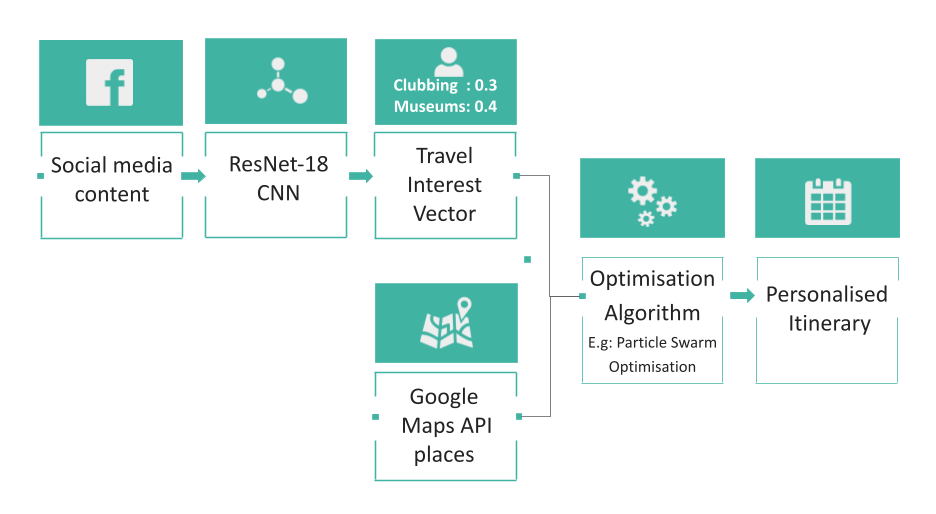
\includegraphics[width=0.6\textwidth]{Methodology.png}
\caption{Personalised itinerary generator}
\label{Methodology}
\end{figure}

%\subsection{Retrieving travel products}

We implemented the Google Maps API as the data source for our application
because of its real-time accuracy and massive dataset compared with the other
approaches and other APIs that we discussed in the literature review
%~\cite{googleSite, iltifat2014generation}. In addition, the nearby search
endpoint allows the app to search
for places of a given category within a specified area. In order to retrieve
the places for the application, eight requests are made, each requesting places
of different categories. To solve the issues with time windows, we split the
endpoints into two categories. Five of the requests represent places shown as
part of the itinerary during the day, and the rest represent places shown
during the night. 

%%TODO: Add figure
%Table X shows the eight categories that were requested. These
%categories are based on the ones used by Wörndl et al.~\cite{Worndl2017} for their
%application.


%In return, the API returns a list of places of the specified area and category
%and attributes about each place. The attributes used by our application include
%the place's name, rating, the number of reviews and the coordinates. All of
%these attributes help the application further optimise the algorithm to find
%the perfect itinerary. 

%%TODO: Add figure
%Figure X shows an example of a response from the API.\



\subsection{Generating the User Profile}
Social media's effect on the world is something significant~\cite{Miller2016}.
That is why this application builds a user profile from
the user's social media. 

The application built by Lim et al.~\cite{Lim2018a} allowed the user to connect
the application with their Flickr profile to scan their past trips. However,
Facebook provides an API that would allow users to connect both their Facebook
and Instagram accounts and request content from the user with their permission.
A significant advantage is that the API allows the
application not to limit the results to mimic only
past user's trips like the application by Lim et al.~\cite{Lim2018a} and gather
preferences from his complete profile.
The app requests two things from the
potential tourist's social media, the photos and the liked pages and tries to
classify these into six categories that make up the user's travel interest
vector; 

\begin{center}
    [   
    1 Beach,
    2 Nature,
    3 Shopping,
    4 Museums,
    5 Clubbing,
    6 Bars ]
    
\end{center}



These categories are the same categories that we requested from the google maps
API except `cafeterias' and `restaurants'. These two categories were not
included because the application tries to suggest the best places to eat as
part of the timetable, irrelevant to the user's profile. At the start of the
application, the app initialises all vector values to zero and increments a
value whenever the user's content matches a category. We will describe how the
app classifies both the user's liked pages and the user's photos separately in
the upcoming subsections.

\subsubsection{Transforming the liked pages into the travel interest vector}

The Facebook API allows the application to request each category of the user's
liked Facebook pages. The API's documentation contains a whole list of possible
categories. 
%TODO: Add Url
%https://www.facebook.com/pages/category. 

The app iterates through
all of these user's likes categories and increments a value in the user's
vector whenever the Facebook result matches one of the six travel interest
vector values. For example, if a user likes a page with class `DJ', the user's
clubbing vector value is incremented, and if a page is labelled as a
`Mountain', the app increments the user's nature vector value.

\subsubsection{Transforming the user's photos into the travel interest vector}


Convolutional Neural Networks have become a standard
for classifying an image because of their high
accuracy~\cite{Zhou2018}. Therefore, we decided to test
out two approaches for classifying the photos into the
app's six categories. 

Zhou et al. \cite{Zhou2018} trained several CNNs for
scene recognition and generic deep scene features for
visual identification. However, the places365 models
are not explicitly trained on the six categories of
our application. Therefore, we need to carefully map
the 365 categories with our six application's
categories. That is why we introduced a Tensorflow
Keras sequential model, explicitly trained on the six
application's categories to compare.

\paragraph{Pretrained Places365 models:} These models
are trained on the places365-standard dataset of about
1.8 million images to classify an image into 365
different scene categories. We used the Resnet
places365 models, Resnet-18 and Resnet-50 since they
achieved the highest top-5 validation accuracy on the
places365 dataset. The Resnet 18 comprises 18, and the
Resnet 50 comprises 50 convolutional layers. They both
converge to an output layer representing the 365
output categories.  Figure \ref{Resnet} shows a
summary of the whole Resnet 18 model.

\paragraph{Trained Tensorflow Keras model: } This
model contains three convolutional layers with a
rectified linear unit (ReLu) activation function. A
pooling layer follows each to lower the input volume's
spatial dimension for the upcoming layers. The final
layer represents a flattening layer and two dense
layers to reduce the outputs to the six application
categories, and another representing the 'None'
classification. Figure ~\ref{Keras} shows a summary of
the whole model. 

\begin{figure}[h]
\centering
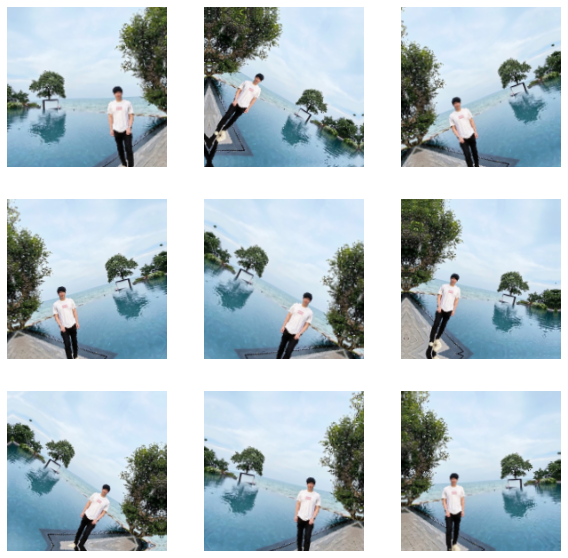
\includegraphics[width=0.3\textwidth]{Augmentation.png}
\caption{Data augmentation to reduce overfitting}
\label{Augmentation}
\end{figure}

The dataset contains 3600 public internet images
representing the seven classes: Beach, Nature,
Museums, Shopping, Clubbing and Bars and None. The
tensor library provides tools to Split the dataset
into a training and validation set Distribute the
photos into batches of 32 Cache the dataset to memory
to prevent I/O blocking All of the images were resized
to 180x180 pixels, and the RGB values were normalised
from zero to one.  	Since the dataset is small
compared to the places 365 models, the training
process is prone to overfitting. Data augmentation
generates additional samples using random
transformations on the dataset. Figure \ref{Augmentation} shows an
example of data augmentation on a photo. We also added
a dropout layer to the model randomly drops sets the
input values of the neuron. These two techniques help
the model avoid overfitting.


\begin{figure}[H]
  \centering
  \begin{minipage}[b]{0.4\textwidth}
    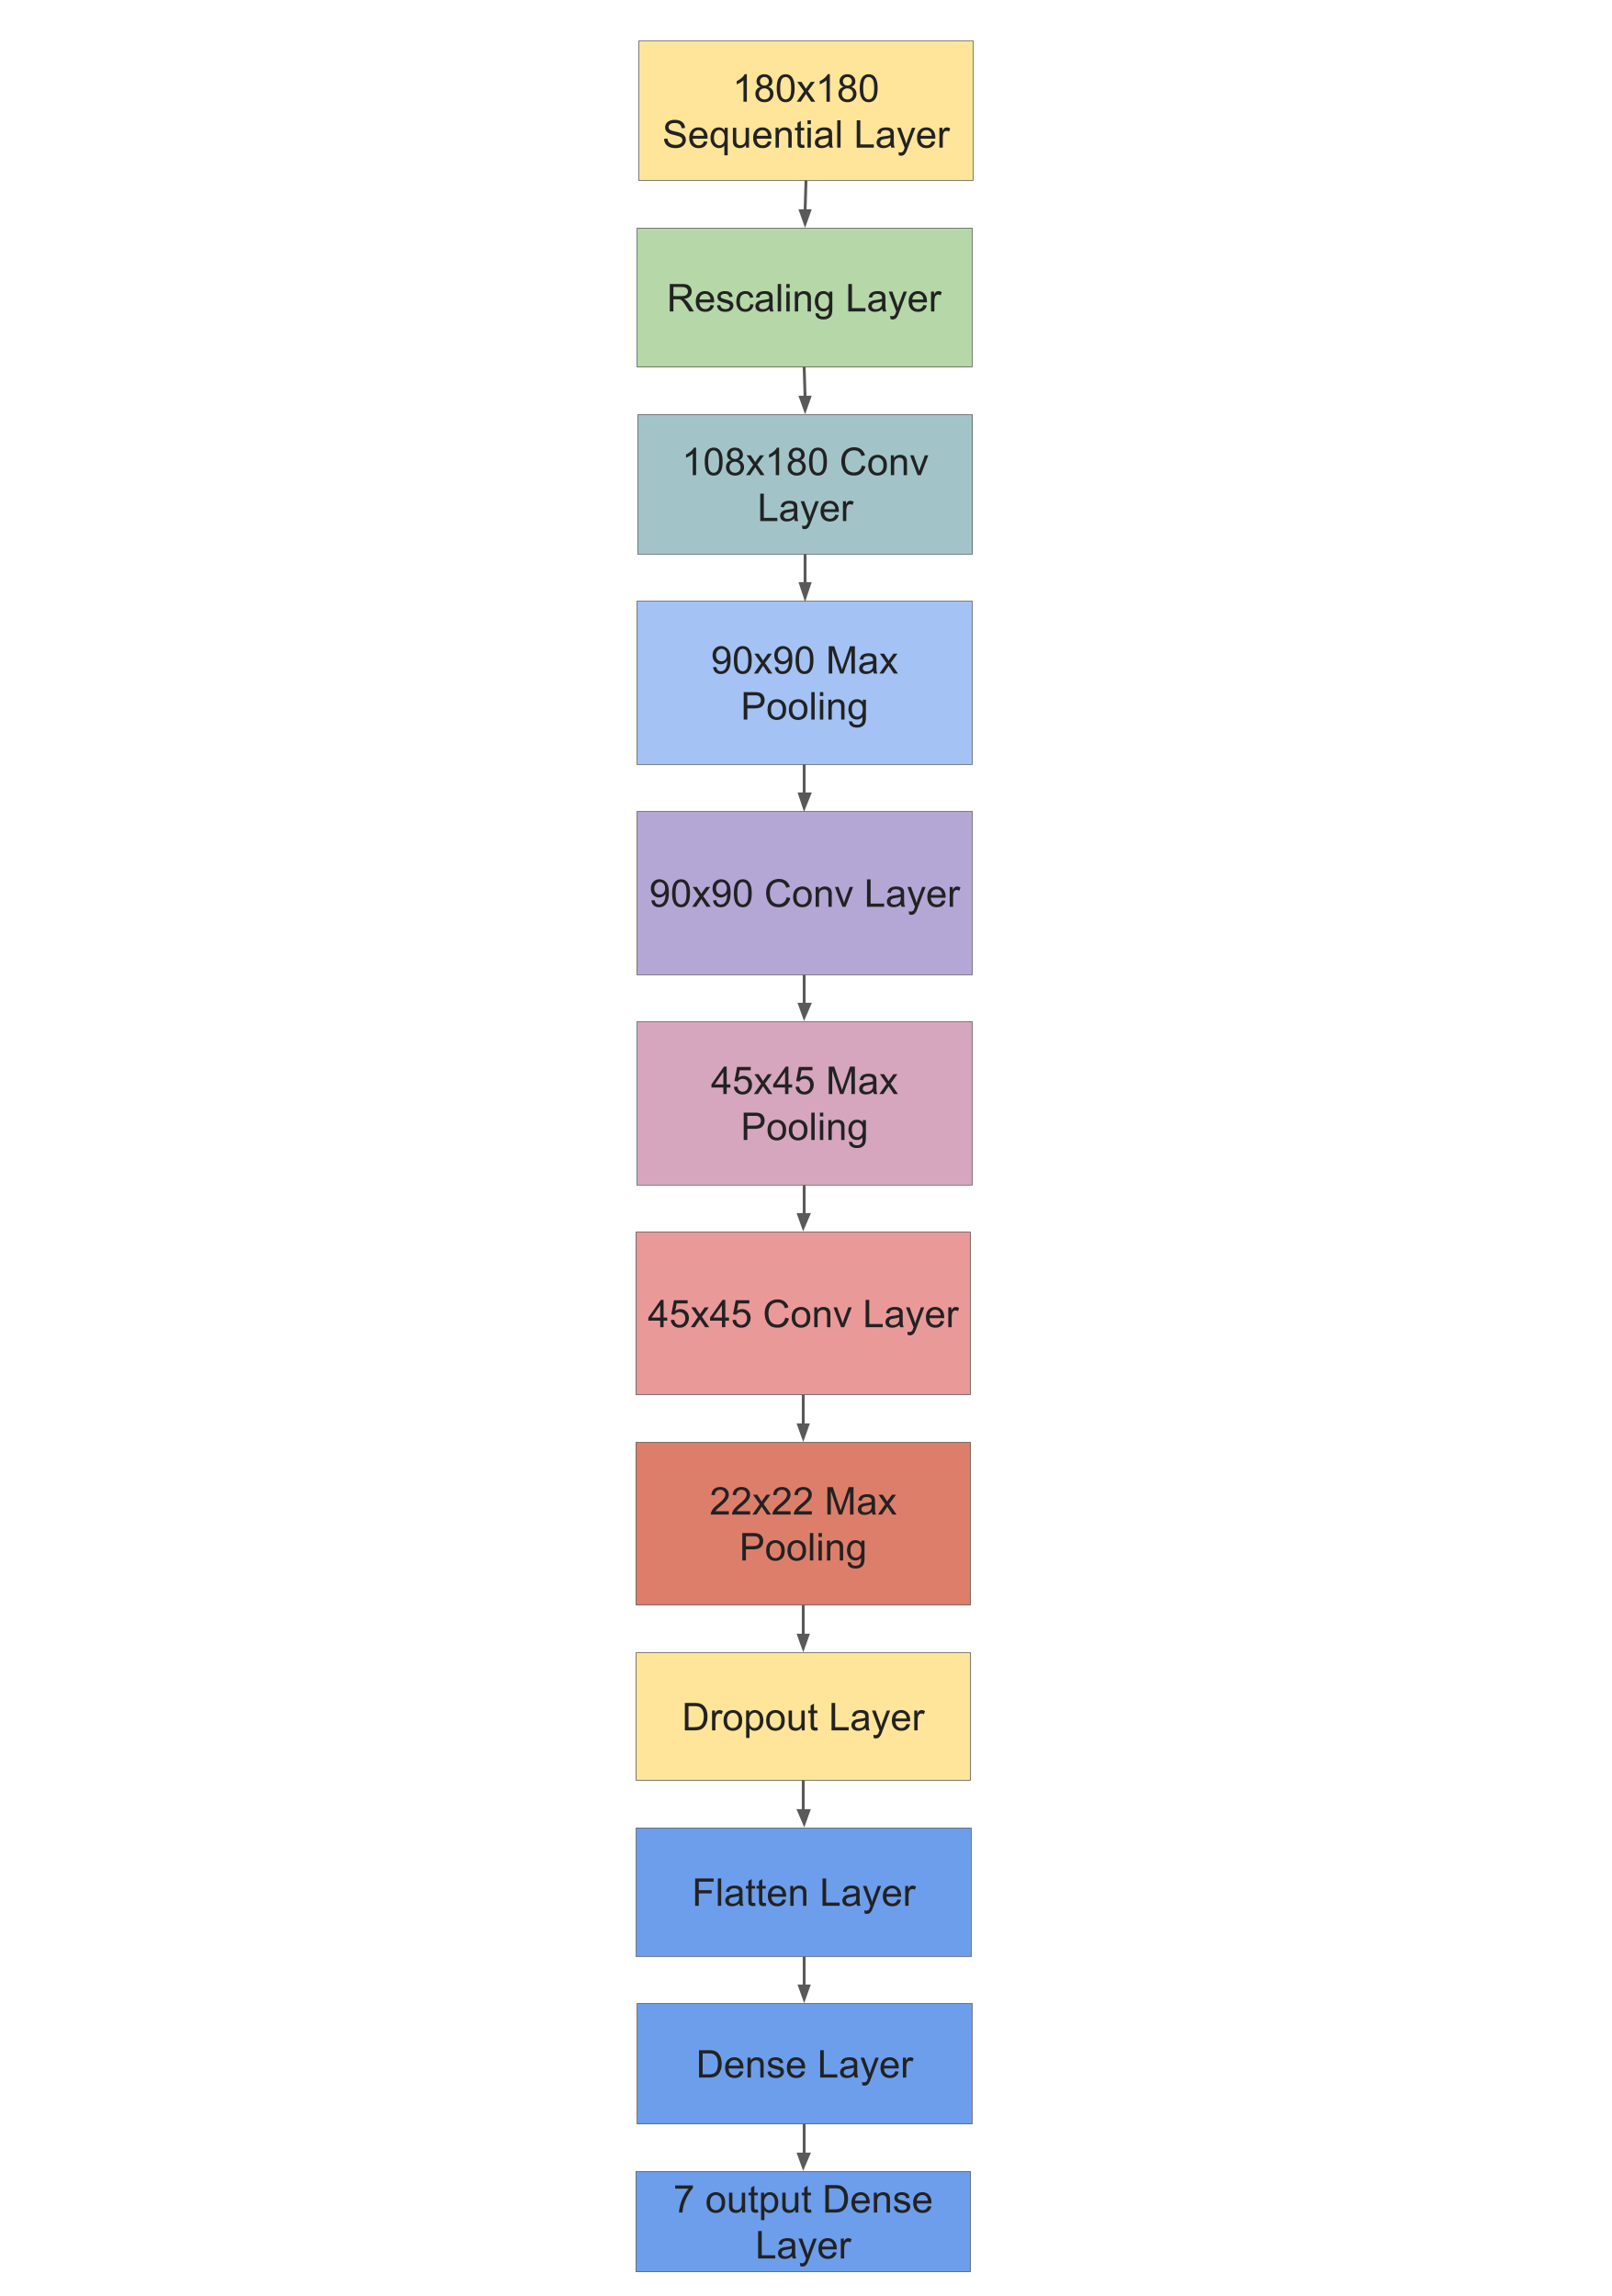
\includegraphics[width=0.8\textwidth]{KerasSequential.png}
    \caption{Keras Sequential Architecture Summary}
    \label{Keras}
  \end{minipage}
  \hfill
  \begin{minipage}[b]{0.4\textwidth}
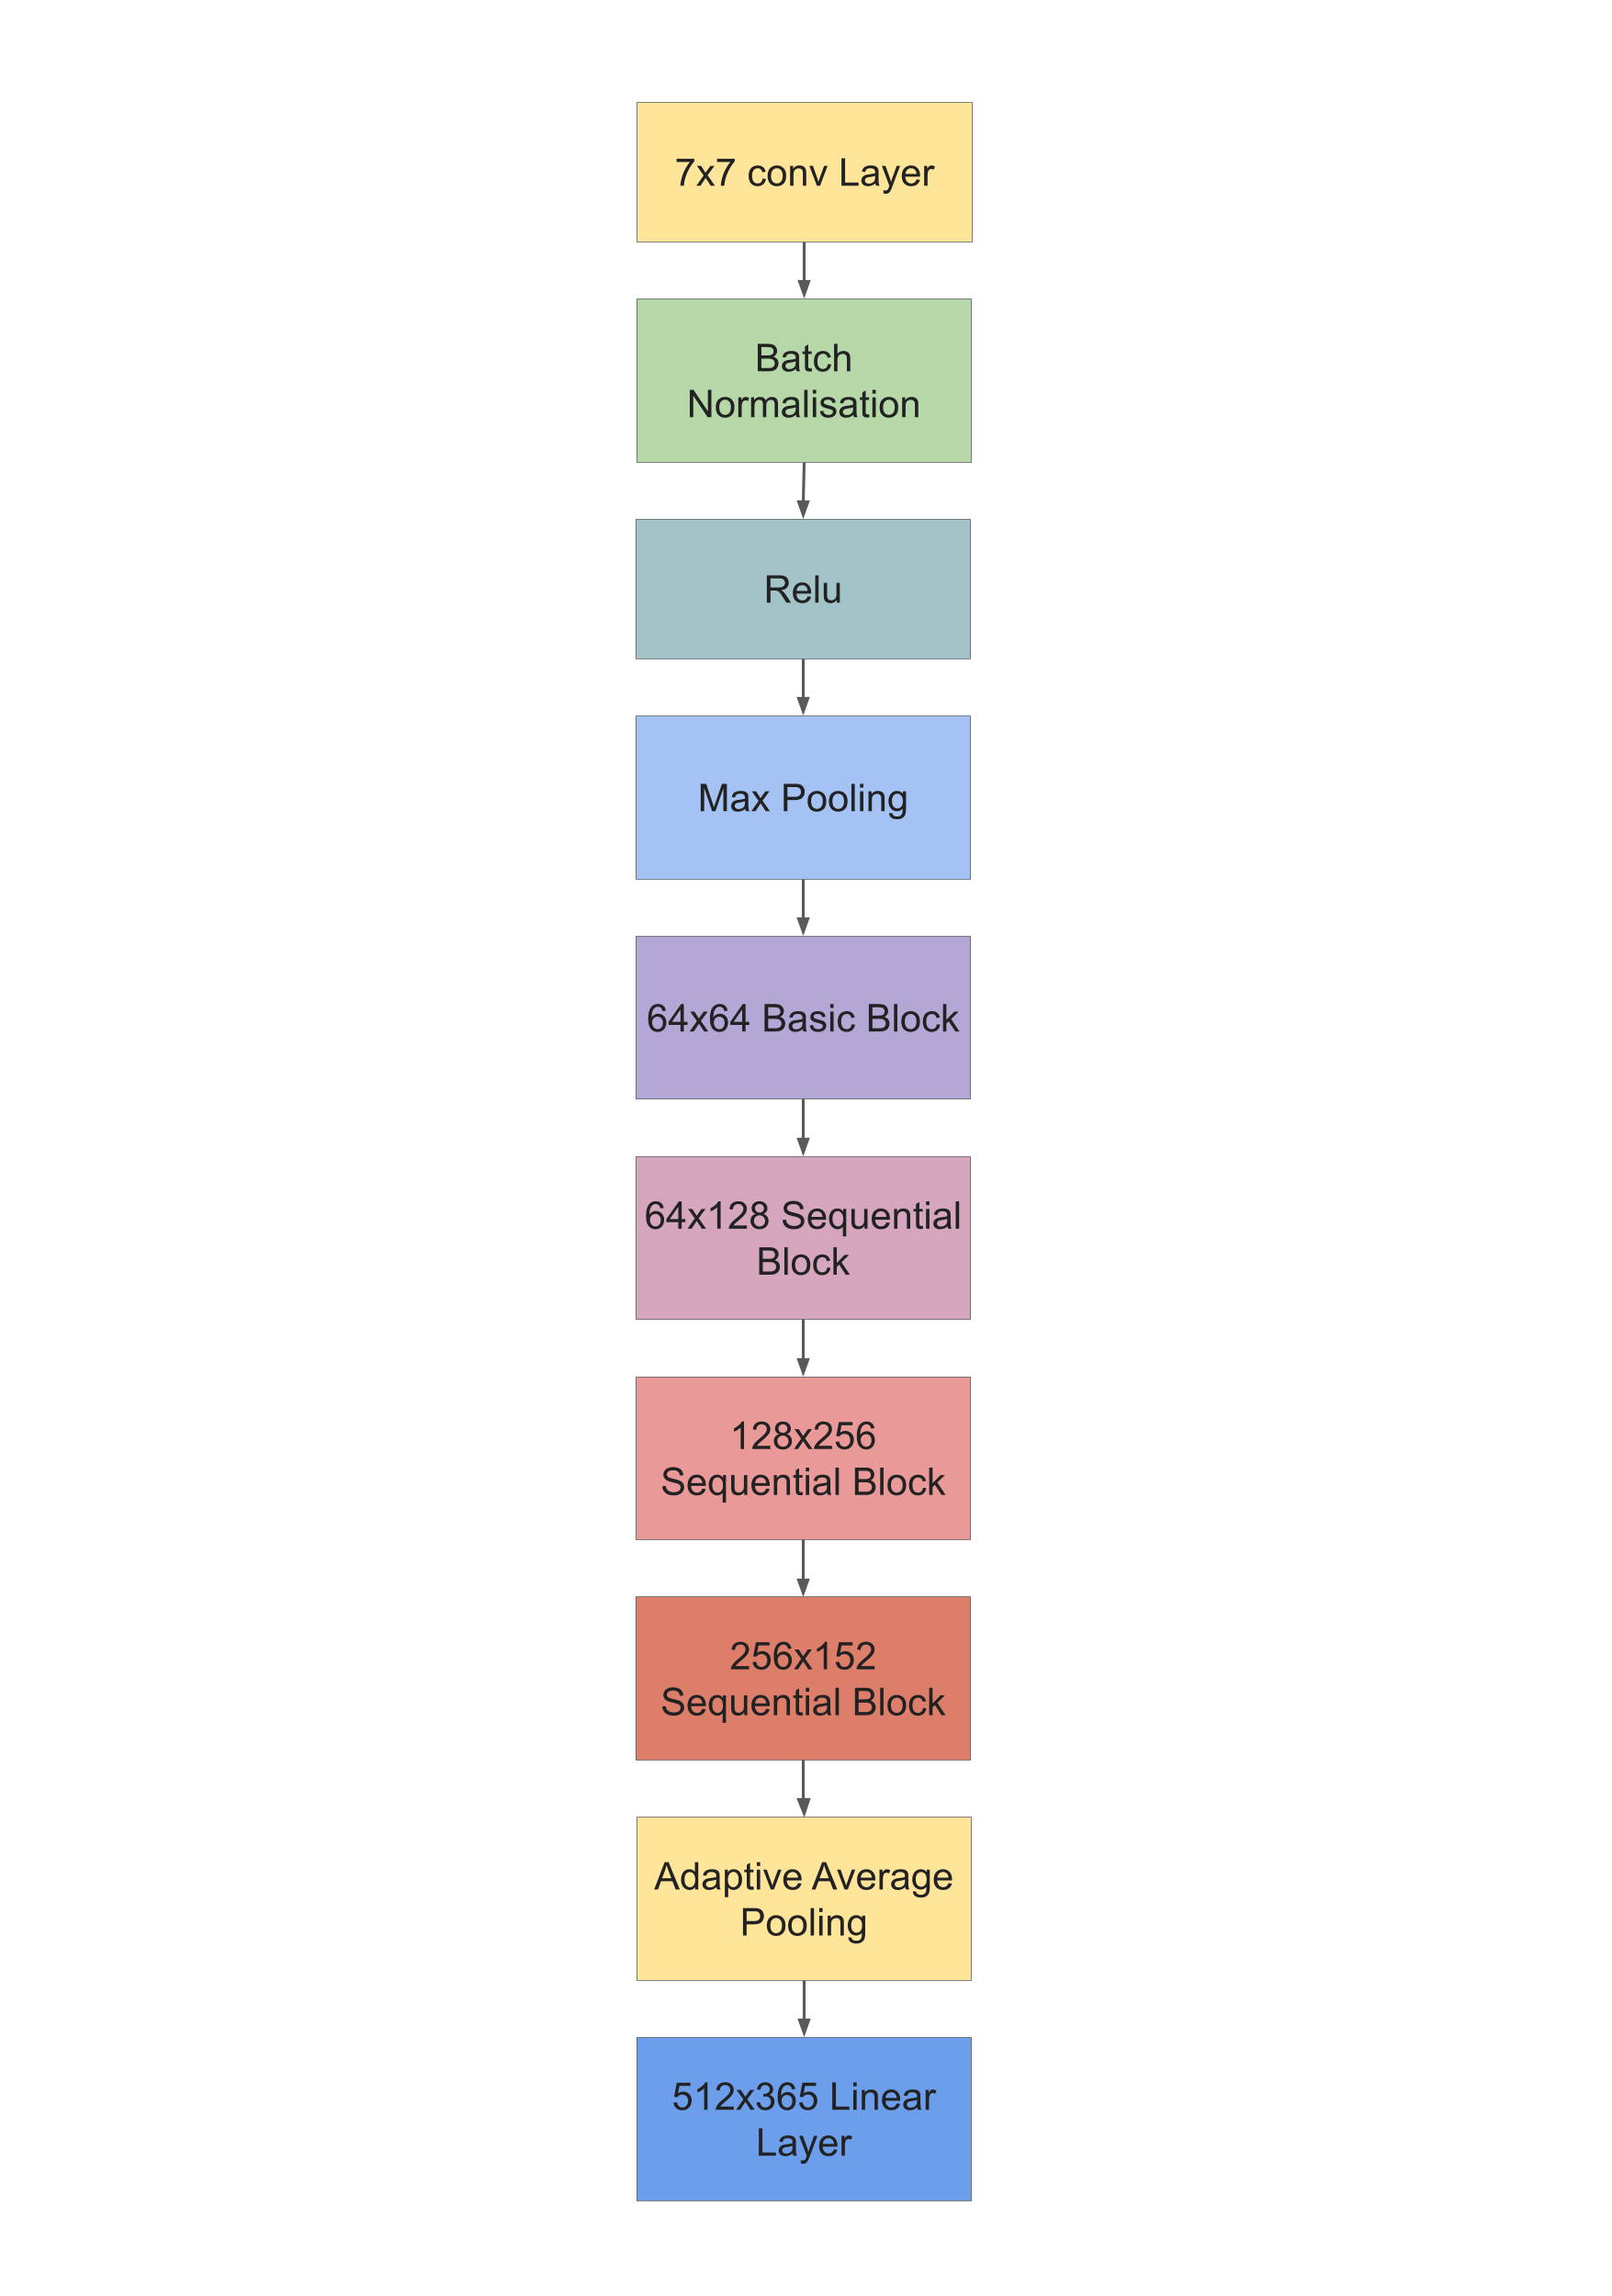
\includegraphics[width=0.8\textwidth]{Resnet.png}
\caption{Resnet 18 Architecture Summary}
\label{Resnet}
  \end{minipage}
\end{figure}



\subsection{Producing the activity plan}

After the app generates the dataset of POIs and the
user's travel interest vector, we formulate an
efficient activity plan using these two inputs. This
itinerary generator is based on the existing state of
the art activity planners~\cite{Sylejmani2017, Wisittipanich2020}
with some adjustments: We wanted the trip's output to take the
form of an itinerary.  The problem takes the form of
the `day' and `night'  category split discussed in
the literature review.  The scoring of itineraries is adjusted
with the travel interest vector.

The problem definition of our novel itinerary planner
is mathematically formulated as follows. A tourist trip is made up
of some pre-defined user constants alongside the travel interest
vector. The predefined constants are:
\\


\setlength{\tabcolsep}{20pt}

\begin{tabular}{l l}

\textit{M}:  &  The number of travelling days \\
\textit{C}: & The activity pace (ie. the greater the \\
 & C value, the more activities are generated in \\
 & a day) \\  
\end{tabular}
\\
\\
\\
The objective function of our itinerary planner is:

\[ \text{MAX}  \sum_{m=0}^{M} ( S_{{D_m}} + S_{{E_m}}) \]
where:
\\
\begin{tabular}{l l}
% \textit{i,j}:  &  POI (\textit{i,j} = 2,3,...,\textit{N}) \\
\textit{m} & Travelling day (\textit{m}=1,2,\ldots, textit{M}) \\ 
\textit{$D_m$} & Morning section of day number m \\  
\textit{$E_m$} & Evening section of day number m \\  
\textit{$S_{D_m}$} & Score of the morning section $D_m$ \\  
\textit{$S_{E_m}$} & Score of the evening section $E_m$ \\  
\end{tabular}
\\
\\

A day is made up of the morning ${D_m}$ section and
the evening ${E_m}$ section. The timetable suggests a
POI in the morning, then somewhere to eat, and the
rest is dependant on the activity pace C. That is why
the morning section is made up of $C + 2$ tourist
attractions. The evening section suggests a place to
eat and a POI; therefore, the evening section is just
made up of $2$. 


\[D_m = Y_i + Y_f + C ( Y_i) \]
\[E_m = Y_f + Y_j \]

\begin{tabular}{l l}

\textit{i} & Morning Tourist attraction (i = 1, 2, 3,…, $n_1$)\\
\textit{j} & Evening Tourist attraction (j = 1,2, 3,…, $n_2$)\\
\textit{f} & Food Place (f = 1,2, 3,…, $n_3$)\\
\textit{$Y_{i|f|j}$}: & 1 if a tourist visit attraction i, j or f and  0 if otherwise\\
\end{tabular}
\\ 
\\
\begin{tabular}{l l}
\textbf{Constraints} & \\
\textit{$ \sum_{m=0}^{M}\sum_{i=0}^{n_1}{Y_i} \leq 1$} & Ensures that all morning tourist attractions are \\ & not visited more than once throughout the whole \\ & itinerary\\

\textit{$ \sum_{m=0}^{M}\sum_{j=0}^{n_1}{Y_j} \leq 1$} & Ensures that all evening tourist attractions are \\ & not visited only once throughout the whole \\ & itinerary\\


\end{tabular}

\subsubsection{Calculation of Score}

The score $S_{D_m}$ or $S_{E_m}$ is calculated using

\[ S_{D_m | E_m} = \frac{1}{T} + R + V\]

where:
\\
\begin{tabular}{l l}
% \textit{i,j}:  &  POI (\textit{i,j} = 2,3,...,\textit{N}) \\
\textit{T} & Total distance between each tourist attractions in the \\ & morning/evening of day m\\ 
\textit{R} & Average rating of the tourist attractions in the \\ & morning/evening of day m \\  
\textit{V} & how much the tourist attractions of the \\ & morning/evening of day m match with the user's \\ & travel interest vector \\  

\end{tabular}
\\
\\


\subsection{Retrieving travel products}

We implemented the Google Maps API as the data source for our application
because of its real-time accuracy and massive dataset compared with the other
approaches and other APIs that we discussed in the literature review
%~\cite{googleSite, iltifat2014generation}. In addition, the nearby search
endpoint allows the app to search
for places of a given category within a specified area. In order to retrieve
the places for the application, eight requests are made, each requesting places
of different categories. To solve the issues with time windows, we split the
endpoints into two categories. Five of the requests represent places shown as
part of the itinerary during the day, and the rest represent places shown
during the night. 

%%TODO: Add figure
%Table X shows the eight categories that were requested. These
%categories are based on the ones used by Wörndl et al.~\cite{Worndl2017} for their
%application.


%In return, the API returns a list of places of the specified area and category
%and attributes about each place. The attributes used by our application include
%the place's name, rating, the number of reviews and the coordinates. All of
%these attributes help the application further optimise the algorithm to find
%the perfect itinerary. 

%%TODO: Add figure
%Figure X shows an example of a response from the API.\



%\subsubsection{}
\subsubsection{Optimisation Algorithms}

The following will discuss the steps required to
produce the two timetable optimisation algorithms. PSO
and GAs are two meta-heuristics that use a population
to converge to a fit solution. Therefore, they require
an initial random generation of possible timetables. In
our algorithm, we introduce a method of randomisation
bias which will be discussed before the algorithms.


\paragraph{Random Bias}
With this technique, the randomness of the initial
population is weighted based on two components.
\begin{enumerate}

    \item  the place's rating and 

    \item the place's number of ratings.
\end{enumerate}


Before the algorithm starts each POI will be given a score 
that will determine its probability of being chosen as
part of the initial population. For example, if a
POI $i$ has a rating, 
$r_i$ which a value from 0 to 5, and
the number of ratings from users $z_i$. The score of $i$
is calculated using the following equation:

    \begin{center}
        score = $\frac{r_i}{5}+\frac{z_i}{\text{max}(\sum_{j=0}^{N}{z_j})}$

    \end{center}
%\[ \text{score} = (p_i)p_i\text{.rating}\]

This bias gives a head start to the algorithm
rather than just starting optimising from purely
random itineraries, highly likely to be of bad
quality.


\begin{algorithm}[h]

 iter = x \;
 count = 0 \;
 particles = RandomBiasInitialiser(); \;
 bestParticle = particle[0] \;

 \While{count $>$ x}{

     i = 0 \;
     maxScore = 0 \;

     \While{i $<=$ particles.length}{

         \tcc{Updating personal best}
        \If{particles[i].score $>$ particles[i].personalBest.score}{

             particles[i].personalBest = particles[i].position\;

         }

         \tcc{Updating global best}
        \If{particles[i].score $>$ maxScore}{


             maxScore = particles[i].score \;
             bestParticle = particles[i].position \;

         }

         i = i +1 \;

         \tcc{Calculate new position}
         particle[i].calculateNewPosition() \;



     }
     \Return bestParticle

 }

 \caption{Particle Swarm Optimisation}
    \label{PSOAlgorithm}
\end{algorithm}



\paragraph{Particle Swarm Optimisation}

In PSO, the whole population is referred to as the
swarm, whilst a single member a particle. Each
particle has a 2-dimensional position(P) vector
representing the current timetable solution and a
2-dimensional velocity(V) vector expressing the direction
of the particle during its search period. 

The algorithm has six integer parameters including the
number of particles and the number of iterations. The
personal acceleration (PA) affects how far away the
particle moves from the personal best position (PB). 
The global best acceleration (GA) attracts the global
best position (GB) of the whole swarm. 
The inertia (I) constant helps the particle
explore new solutions and escape the local minima
through randomness. 

At each
iteration, the new velocity is calculated using
\begin{center}
    new velocity = I + (PA * (PB - P)) + (GA * (GB - P))
\end{center}

the new position is calculated using
\begin{center}
    new position = P + new velocity 
\end{center}

After a few iterations have passed, particles use
their velocity and move towards the optimum position.
We demonstrate the framework of our PSO algorithm in
algorithm \ref{PSOAlgorithm}.


\paragraph{Genetic Algorithms}

Genetics algorithms use biological terms to describe
their attributes. For example, a timetable solution in
population is referred to as a chromosome. (cite) 

In PSO, the algorithm optimises by allowing each
particle to move closer to the global best every
iteration. In comparison, in GAs, first, the best
chromosomes known as the elites are selected from each
iteration. Then, three techniques, namely selection,
mutation, and crossover, are applied to generate the
next population.

We used the geneticalgorithm2 package provided by X,
which allowed us to use the same score function and
the random bias to initialise the particles. The
algorithm has X parameters. The parents portion
represents the number of parents who will reproduce
and create the next generation. The mutation
probability determines the chance a POI in a
chromosome will be replaced by a random value to which
the algorithm will converge less quickly and explore
more of the search space. The crossover probability
will affect the chance that part of its solution goes
to the child. Finally, the elite ratio determines how
much of the best chromosomes in an iteration make it
to the next iteration.  There are many types of
crossovers and mutations. In this algorithm, we
explored X.  The algorithm produced the following
steps: \\
\textbf{Step 1}: Initialise the first population using random bias. \\
\textbf{Step 2}: Select the best chromosomes from the population. \\ 
\textbf{Step 3}: Select the elite particles that will make it to the next iteration.\\
\textbf{Step 3}: Apply Crossover, Mutation and Selection on the population. \\
\textbf{Step 4}: Check if the number of iterations has exceeded. 






\pagebreak

\section{Results and Evaluation}

This section will evaluate the image
classification technique for the automatic user profiling and the itinerary
generation algorithm separately. We will then assess the performance of the
whole application and the effect of automated personalisation through in-depth
semi-structured interviews with users experiencing the website.


\subsection{Automatic User Profiling} 

The following evaluates the performance results of the
three CNNs used to classify the users' social media images.

\paragraph{Training results from the TensorFlow Keras sequential model}

We trained this model using the NVIDIA Tesla K80 GPU provided by Google Colab. At 16 epochs,
the model starts to overfit as the validation loss starts to increase, as shown
in figure~\ref{kerasresults}. This is why we chose to calculate the model's performance on the
testing set in the following subsections using the first 16 epochs. 

\begin{figure}[h]
\centering
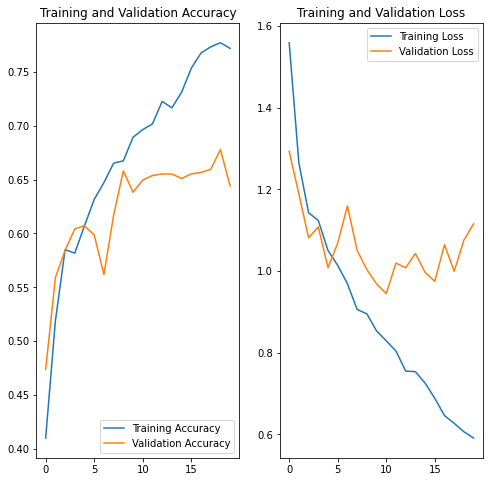
\includegraphics[width=0.6\textwidth]{Epoch_20.png}
\caption{Training and validation accuracy of the model on the testing and validation dataset}
\label{kerasresults}
\end{figure}

\paragraph{Performance comparison of the three models}

The testing dataset consists of 500 images manually gathered using the Unsplash API. We
calculated the Accuracy, Precision, Recall and F1 Score on the testing set to
evaluate the models by calculating the number of true positive (TP), true
negative  (TN), false-negative (FN) and false positive (FP) as a
percentage over the dataset. 

The accuracy of the models, shown in figure~\ref{accuracy}, is represented by:

\[Accuracy = \frac{TP+TN}{TP+FP+FN+TN} \]

This shows how many category predictions a model got right. In this case, the Resnet 50,
Resnet 18, and Keras models have an average 93.7\%, 92.4\%, and 88.7\% average accuracy,
respectively. Overall, the models have high accuracy. Therefore, we need to rely on other
evaluation techniques.

\begin{figure}[h]
\centering
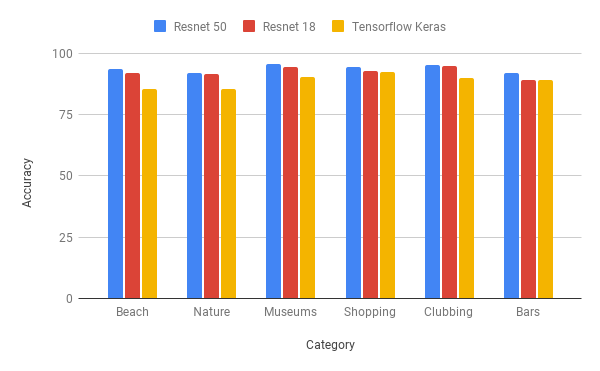
\includegraphics[width=0.7\textwidth]{Accuracy.png}
\caption{Accuracy of the models}
\label{accuracy}
\end{figure}

The precision of the models, shown in figure~\ref{precision}, represented by

\[Precision = \frac{TP}{TP+FP} \]
This represents the ratio of correct predictions over the total positive labels.
In this case, the Resnet 50, Resnet 18, and Keras models have an average 72.4\%, 66.7\%,
and 62.4\% precision rate, respectively. The Resnet 50 has the best average
overall; however, the Keras model performed better for the 'clubbing' and
'bars' categories but very poorly in the shopping category.

\begin{figure}[h]
\centering
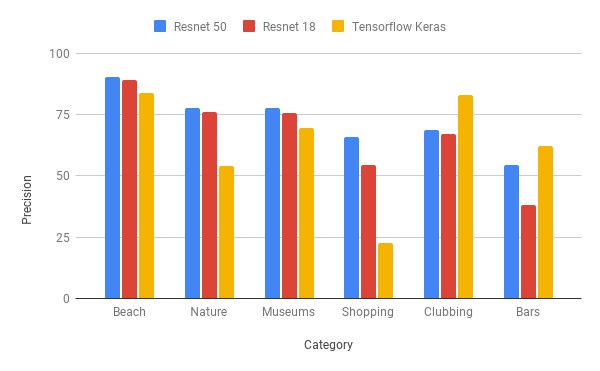
\includegraphics[width=0.7\textwidth]{Precision.png}
\caption{Precision of the models}
\label{precision}
\end{figure}

The proportion of actual positive labels that the models identify correctly is
represented by the recall value calculated using 

\[Recall= \frac{TP}{TP+FN} \]

In this case, figure \ref{recall}
shows how for the clubbing and bar categories, although the Resnet models were
less accurate and less precise, they rarely labelled an image as a bar or a
club when they are not supposed to.

\begin{figure}[h]
\centering
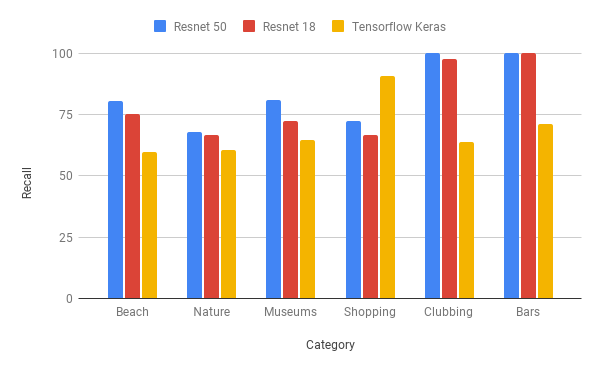
\includegraphics[width=0.7\textwidth]{Recall.png}
\caption{Recall of the Resnet-18, Resnet-50 and Tensorflow Keras Sequential}
\label{recall}
\end{figure}

The F1 score is the weighted average of Precision and Recall measured using:

\[F1 Score = \frac{2*Recall*Precision}{Recall+Precision}  \]
The Reset 50 has a pretty consistent and high score on
the testing dataset with an average F1 score of 76.29., so
we decided to use it as our baseline for the tourist
itinerary generation application.

\begin{figure}[h]
\centering
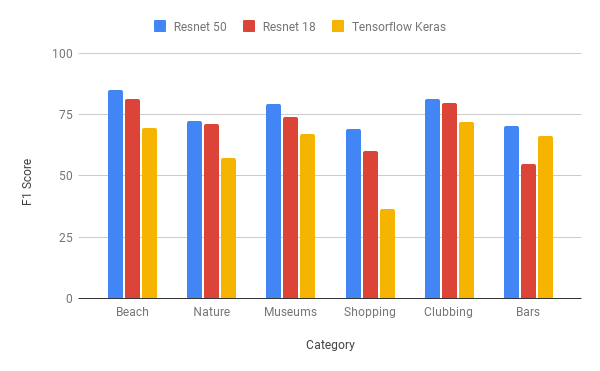
\includegraphics[width=0.7\textwidth]{F1Score.png}
\caption{F1 score of the Resnet-18, Resnet-50 and Tensorflow Keras Sequential}
\label{f1}
\end{figure}

These results have shown how a CNN could classify photos into the six
application characteristics. Although all of the models achieved valid results,
the Resnet 50 model was the best performer. Therefore, we will be using this
model for our application.

\subsection{Itinerary Optimisation Algorithms}

We tested out the itinerary generation algorithm using
POIs in Malta. The algorithm has to optimise to
produce the best itinerary for X number and several
tourist constraints. Figure \ref{optimise} shows the score of 10
PSO itineraries increasing throughout several
iterations for the morning and evening section of the
day.

\begin{figure}[h]
\centering
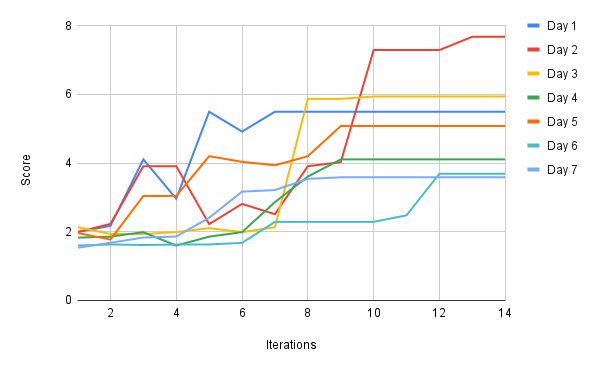
\includegraphics[width=0.7\textwidth]{Optimisation.png}
\caption{Training and validation accuracy of the model on the testing and validation dataset}
\label{optimise}
\end{figure}

Many parameters help tweak the performance of the PSO
algorithm. The population size and the number of
iterations are the two main attributes of the PSO
algorithm. At around 12 iterations in figure~\ref{optimise}, the
algorithm generally converges. Figure X shows the
spread of particles converging. 


Increasing the number of particles also increases the
average score, as shown in figure~\ref{score} for 10 generated
itineraries and 14 iterations. However, the difference
in average score between 50 and 100 particles is not
proportional to the average time taken to create an
itinerary for a single day in figure~\ref{time}.  That is why
for the application, the population is set to 50. 

\begin{figure}[h]
\centering
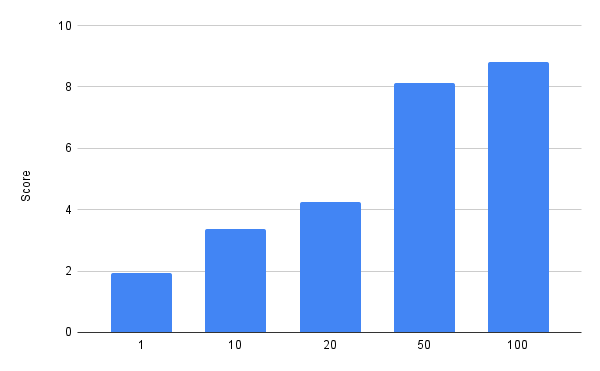
\includegraphics[width=0.7\textwidth]{Score.png}
\caption{Training and validation accuracy of the model on the testing and validation dataset}
\label{score}
\end{figure}

\begin{figure}[h]
\centering
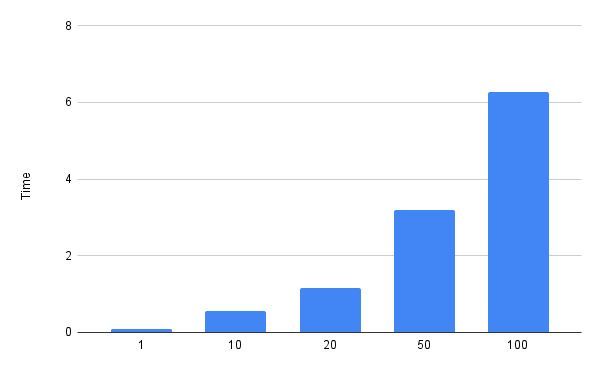
\includegraphics[width=0.7\textwidth]{Time.png}
\caption{Training and validation accuracy of the model on the testing and validation dataset}
\label{time}
\end{figure}

The original algorithm X did not contain the inertia
property; however, it was introduced by X since it
controls the convergence behaviour. Out algorithm
implements the Time-Varying Inertia Weight X, which
gradually decreases throughout each iteration. Figure
X shows the optimisation algorithm without the inertia
property and barely increases the score since the
particles do not explore new territories.


\pagebreak

\section{Conclusion and Future Work}

In this dissertation, we addressed the question `Can a system automatically
recognises a tourist's travel preferences and use this information to generate
a personalised itinerary for a holiday?'. 

We introduced an automatic preference gathering technique that scans a user's
social media profile and analyses the user's photos and liked pages. Our work
presents a comparison between three CNNs: the Resnet 18, Resnet 50 and Keras
Tensorflow models trained to classify an image into one of the following user
characteristics; Beach, Nature, Shopping, Museums, Nature Clubbing and Bars.

As a result, we have built an application to solve the TTDP that considers the
popularity of POIs, the user's automatically generated interests, the user's
activity pace and the distance between places as constraints to recommend a
suitable itinerary.

We optimised the timetables by comparing two meta-heuristics, Particle Swarm
Optimisation and Genetic algorithms and found that the PSO algorithm provided
the best balance between achieving the highest score and providing the solution
in a reasonable amount of time. 

Finally, we asked 20 people to provide us with feedback regarding the
personalisation of the timetables through in-depth semi-structured interviews.
The interviews displayed personalised results and non-personalised results in
random order, and without informing the interviewees which one was which, 15
people prefered the personalised itinerary.

So far, we used the user's photos and the user's liked pages to gather the
preferences automatically. However, we have seen through the interviews that not
everyone feels that what they post online represents their travel preferences.
Therefore, more diverse approaches through social media should be applied and
compared in future work such as:

\begin{itemize}
\item Gather characteristics from social media contacts that potential tourists follow.
\item Use Natural Language Process techniques to scan the user's online posts.
\item Expand the application to use other social media APIs such as Twitter and Google Photos to reach more people. 
\end{itemize}

Although there is always room for further development, this dissertation forms
the basis to prove that an automatic preference gathering system can further
assist a travel-related application to achieve more satisfactory results for
its users.


\pagebreak

\bibliographystyle{IEEEtran}
\bibliography{/home/liam/Documents/latex/library/bibFile/library.bib}


\pagebreak
\section{Table of Interview Results}



\begin{figure}[h]
    \centering
    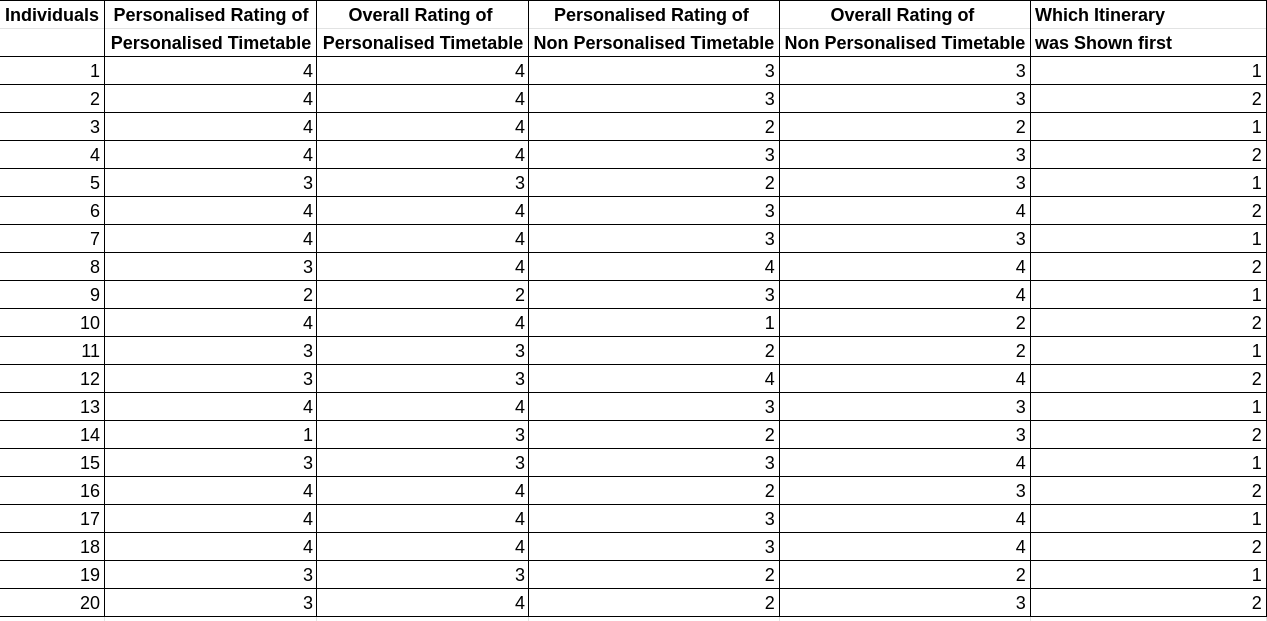
\includegraphics[width=0.9\textwidth]{ScoreOne.png}
\end{figure}

\begin{figure}[h]
    \centering
    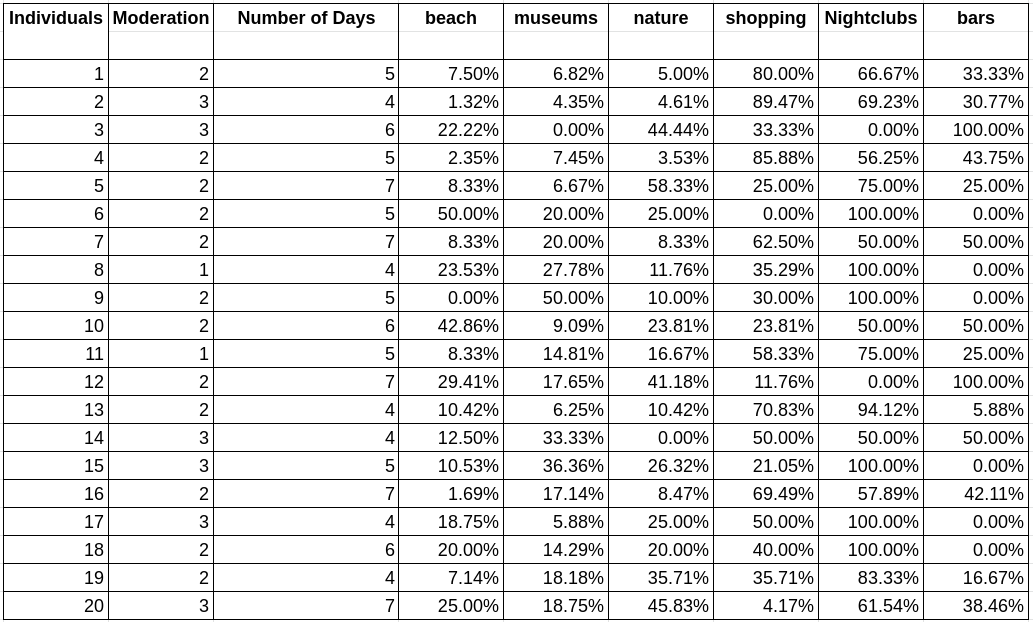
\includegraphics[width=0.9\textwidth]{ScoreTwo.png}
\end{figure}

\pagebreak

\end{document}

